\documentclass[a4paper,11pt]{report}
\usepackage{graphicx}
\usepackage[backend=bibtex]{biblatex}
\usepackage{pgfplots}
\usepackage[strings]{underscore}
\usepackage[T1]{fontenc}
\usepackage{amsmath}
\bibliography{dissertation}

\addtolength{\oddsidemargin}{-.7in}
\addtolength{\evensidemargin}{-.7in}
\addtolength{\textwidth}{1in}

\addtolength{\topmargin}{-.7in}
\addtolength{\textheight}{1in}

\usepackage{titlesec}
\titleformat{\chapter}[hang]
{\normalfont\Huge\bfseries}{\chaptertitlename~\thechapter:}{10pt}{\Huge\bfseries}
\titlespacing{\chapter}{0pt}{20pt}{10pt} 
\titleformat*{\section}{\LARGE\bfseries}
\titleformat*{\subsection}{\Large\bfseries}
\titleformat*{\subsubsection}{\large\bfseries}
%\titlespacing*{\chapter}{0pt}{40pt}{40pt}
%\titlespacing*{name=\chapter}{0pt}{40pt}{10pt}

\begin{document}
\begin{titlepage}
	\centering
	
\includegraphics[scale=0.9]{images/cslogo.png} % also works with logo.pdf
	\vfill
	{\bfseries\Huge
		Building a Lambda Expression Evaluator as a Learning Support Tool\\
	}
	\vskip2cm
	{\huge
		Yola Jones\\
	}
	{\LARGE
		\vskip0.5cm
		2409217J\\
		\vskip0.75cm
		Supervisor: Ornela Dardha
	}
	\vskip2cm
	{\Large
		September 2019\\
		\vskip1cm
		A dissertation presented in part fulfilment of the requirements of the degree of MSc in Software Development at the University of Glasgow
	}  
	\vfill
	
	
%\centering
%
\includegraphics[scale=0.75]{images/cslogo.png}
%\title{Building a Lambda Expression Evaluator as a Learning Support Tool}
%\author{Yola Jones (2409217J)}
%\date{\today}
\end{titlepage}
\thispagestyle{empty}
\begin{abstract}
This dissertation describes the design, implementation and evaluation of a lambda calculus expression evaluator built using ANTLR and contained within a web interface, designed as support material for the Theory of Computation course at the University of Glasgow. This dissertation discusses in detail the relevant sections of lambda calculus as covered on the course, then discusses the process of using Abstract Syntax Trees to examine the structure of a term based on a particular syntax, which can then be used to parse and evaluate input expressions. The approach taken to evaluation using ANTLR has also been discussed in detail, before giving a summary of testing done and evidence to support the statement that the goals of the project have been met.
\end{abstract}
\newpage
\addtocontents{toc}{\protect\thispagestyle{empty}}
\tableofcontents
\newpage

%\maketitle

%
% 	WHAT TENSE IS THIS
%
\renewcommand{\cleardoublepage}{}
\renewcommand{\clearpage}{}
\setcounter{page}{1}
\chapter{Introduction}
Lambda calculus is often reported as being the worlds smallest programming language \cite{Michaelson2011} expressing terms as mathematical functions which can represent any computable problem \cite{Selinger2013}. Students on the Theory of Computation course taught at The University of Glasgow learn lambda calculus to give them an understanding of functional programming and other programming paradigms \cite{CourseSpecification}.\\

This report will cover the work done in producing a web application which will verify and evaluate lambda calculus terms input by a user, in order to support future students learning functional programming. The project has been split into three major tasks:

\begin{enumerate}
	\item Understand and use ANTLR to create a parser which will read lambda terms and produce an abstract syntax tree from the user input
	\item Write a program which will use this tree to find the result of the incoming lambda term
	\item Create a web interface which will allow users to input lambda calculus terms and have them checked and evaluated, in order to aid their understanding of lambda calculus
\end{enumerate}

Since the focus is the Theory of Computation course, learning outcomes and course material have been analysed in order to produce a tool which accurately reflects what is taught. An effort has been made however to make the tool accessible to those learning lambda calculus through different means, for example self teaching or those at other universities. This has resulted in an interface which is aimed at supporting the lecture material but not limited by it, with goals of future work aimed at expanding the interface further to support alternative notation than what is covered in the lectures.\\

Overall the project was a success, an interface was created which accurately evaluates lambda terms through a web interface. The tool implements simply typed applied lambda calculus as taught in the lecture slides, while not requiring users to enter types or functions for those on alternate courses. It also allows for different reduction strategies for those who want a more in depth understanding, wrapped in a simple and clear layout that is easy to use. User testing found that participants enjoyed the interface and said they would use such an interface if they were learning lambda calculus, reporting a significant increase in understanding having used the interface for a short time. The tool created for this project will be given to students on the Theory of Computation course when it it is next taught at the University of Glasgow, in the hopes that it will aid understanding by giving students practical support.\\

The following report documents the process in creating such a tool, by introducing key concepts and literature and refining specific project objectives, then expanding on the design and implementation stages, before finally documenting the testing process and evaluating whether or not the goals of the project have been met.\\

\chapter{Background}
\section{Lambda Calculus}

Lambda calculus is a formal syntax for expressing computation statements as mathematical expressions \cite{Selinger2013} created by Alonzo Church in 1936 \cite{Barendregt2000}. It is an extremely simple model of computation, while still being Turing complete \cite{Rojas1998} and forms the basis for functional programming languages like Haskell \cite{Barendregt2000}. Pure lambda calculus terms are comprised of three elements, variables (such as x or y), abstractions (with one input and one output, in the form $\lambda$x.M) and applications (in the form MN) \cite{Hankin2004}.\\

Applied lambda calculus expands this notation, adding constants which act as values and operations \cite{Slonneger1995}. Typed lambda calculus extends this further, adding types to each term, allowing us to restrict the operations available to different types of objects and ensuring that our expression is runnable \cite{Loader1998}. The combination of applied and typed lambda calculus gives us a grammar which can be used for type checking and arithmetically evaluating lambda calculus terms.\\

The Theory of Computation course teaches simply typed lambda calculus (applied lambda calculus with types), and includes lectures on alpha conversion and beta reduction, alongside the definition of normal form and typing rules. As a result, these will be covered in the following sections in an attempt to use lecture material to define requirements of the final system.

\subsection{Basic Principles}

As discussed above, the lambda grammar is made up of three elements: variables, abstractions, and applications. Abstractions are representations of single input functions, which take one input, and use this input to compute one output. An example abstraction $(\lambda x.x+1)$ is equivalent to the function $f(x) = x+1$, taking one input $x$, and returning the value of $x$ incremented by 1. Multi-input functions can be expressed in nested abstraction terms, for example $f(x,y)=x+y$ in strict lambda notation becomes $\lambda x.\lambda y.x+y$.\\

Applications take abstractions and apply other lambda terms to them using substitution. In a term $(\lambda x.M)N$, substitution takes all the instances of the bound variable x and replaces them with the incoming variable N, or expressed mathematically as $(\lambda x.M)N=[N / x]M$, and happens at the abstraction level.\\

With abstractions, applications and variables, any computable function can be expressed. Functions and constants in applied lambda calculus simplify this slightly, allowing the number one to be expressed as the integer 1 rather than the Church Numeral encoding $\lambda f.\lambda x.fx$ in lambda calculus \cite{Tarau2017}.

\subsection{Alpha Conversion}

Complexity is increased when having applications of variables to abstractions. The lambda term $\lambda x.\lambda y.yx$ multiplies the first input to the function with the second, the point here is that x and y are distinct, different terms. Applying y to this function would result in the application $(\lambda x.\lambda y.yx)y$ which reduces to $\lambda y.yy$, the mathematical representation of multiplying the input by itself. This is incorrect, the meaning of the function has been changed because of the letter chosen to act as the input, and is an example of variable capture.\\

Alpha equivalence is the notion in lambda calculus that the choice of variable names does not matter, $\lambda y.y$ is alpha-equivalent to $\lambda a.a$. This notion is used to prevent variable capture through a process called alpha conversion, the process of comparing the incoming variable to the terms inside the abstraction and changing variable names to eliminate capture.\\

De Bruijn notation is an alternative method of handling this issue, eliminating the need for variables altogether and instead expressing abstraction terms as an index representing which abstraction scope they refer to \cite{Kamareddine2000}.\\

The Barendregt Convention assumes bound variables are suitably chosen to avoid capture, a convention which is taught in the Theory of Computation course. From this and alpha conversion, a set of rules for substitution can be created which rename terms to avoid variable capture as substitution is taking place, defined as follows \cite{Acar2008}:

\begin{equation}
[t/x]y=\begin{cases}
t & \text{if $y=x$}\\
y & \text{if $y\ne x$}
\end{cases}
\end{equation}

\begin{equation}
[t/x](t_1t_2)=[t/x]t_1[t/x]t_2
\end{equation}

\begin{equation}
[t'/x](\lambda y.t)=\begin{cases}
\lambda y.t & \text{if $x=y$}\\
\lambda z.[t'/x][z/y]t & \text{if $x\ne y \land z\notin FV(t) \cup FV(t')$}
\end{cases}
\end{equation}

\subsection{Reduction}

A formal method for evaluating lambda terms is known as a reduction, of which there are different levels which each perform different operations. Alpha conversion (or alpha reduction) \cite{Horowitz2013} is the process of renaming variables to avoid variable capture. Beta reduction focuses on finding the result of applications, discussed below. Delta reduction applies functions to constants arithmetically. Finally, eta reduction takes the output of delta- or beta-reduction and removes any leftover abstraction term in an attempt to simplify the final result \cite{Sookocheff2018Eta}. Not all of these reduction steps are necessary, but each simplifies the term in some way, terminating with a final result.

\subsubsection{Beta Reduction}

Following alpha conversion, beta reduction is ready to be performed abiding by the Barendregt Convention. A definition is first needed which states when a lambda term has reached its simplest form and can be evaluated no further. This is known as the Normal Form of a lambda term \cite{Barendregt2000}, and is defined as a term with no beta-redex \cite{Hudak2008} or which contains no subterms of the form $(\lambda x.M)N$ \cite{Hankin2004}. As previously stated, beta reduction is the process of finding the result from the application of a function, and can be performed by following a number of rules \cite{Gay2019}.

\begin{enumerate}
	\item $(\lambda x.M)N = [N / x]M$
	\subitem $(\lambda x.M)N$ is equal to M with all instances of x replaced by N (substitution)
	\item $M = M$
	\subitem A term is equal to itself
	\item $\frac{M=N}{N=M}$
	\subitem If $M=N$ then $N=M$ through symmetric equality
	\item $\frac{M=N \quad N=L}{M=L}$
	\subitem If $M=N$ and $N=L$ then $M=L$ through transitivity
	\item $\frac{M=N}{MZ=NZ}$ and $\frac{M=N}{ZM=ZN}$
	\subitem If $M=N$, then Z applied to M is the same as Z applied to N. Similarly if $M=N$ then M applied to Z is the same as N applied to Z
	\item $\frac{M=N}{\lambda x.M = \lambda x.N}$
	\subitem If $M=N$, then $(\lambda x.M)$ = $(\lambda x.N)$
\end{enumerate}

Different choices made in the application of these rules can generate different results. A fundamental theorem in the world of lambda calculus is the Church-Rosser theorem, and leads to a useful axiom: a term in the lambda calculus has at most one normal form \cite{Alonzo1936} meaning different reduction strategies cannot produce different normal forms. However, if a lambda term does have a normal form, not all methods of reduction reach it \cite{Horowitz2013}.\\

The Theory of Computation course teaches two approaches to beta-reduction, call-by-value and call-by-need. Call-by-value is a leftmost innermost strategy, \cite{Gay2019}, meaning in a term MN, M gets reduced to its normal form before N (the left term is reduced first). In a term $(\lambda x.M)N$, N is evaluated before it gets substituted into $(\lambda x.M)$. For this reason, call-by-value is sometimes referred to as applicative order reduction, as the arguments are reduced before they are applied \cite{Sookocheff2018Evaluation}.\\

Call-by-need is similar but with one key difference, rather than reducing N and then substituting the result into M, the original N is substituted into M before $[N / x]M$ is reduced together as a whole. This is a subtle but very important difference, call-by-need can be proven to always turn a lambda term into its normal form if one exists \cite{Horowitz2013}, unlike call-by-value. Because of this property, call-by-need is often referred to as normal-order-reduction.

\subsection{Typing Rules}

A desirable property in software engineering is static checking at compile time. This can be done with lambda calculus by introducing types, which can be used to verify a lambda term is performing valid computations before being evaluated arithmetically. For example, the lambda term $(\lambda x.x+1)y$ is a valid term, but is not feasible if y is a boolean value such as TRUE or FALSE.\\

To use this, a type definition is first needed. A type T can be of ground type A (boolean or integer), or function type T$\rightarrow$T (taking a type T, and converting it into another type T through a function) \cite{Gay2019}. In order to type-check the validity of a lambda term, a typing context $\Gamma$ is expressed which declares a set of variables to be associated with specific types. From this, three typing rules can be expressed \cite{Gay2019}:

\begin{itemize}
	\item For variables, if x of type T belongs to the typing context $\Gamma$, in $\Gamma$, x is of type T:
	
	\begin{equation}
	\centering
	\frac{x:T\in \Gamma}{\Gamma \vdash x:T}TVar
	\label{variable_type}
	\end{equation}
	\item For abstractions, if in a typing context $\Gamma$ where x has type T, if M has type U, then $\lambda$x.M has type T $\rightarrow$ U:
	
	\begin{equation}
	\centering
	\frac{\Gamma ,x:T\vdash M:U}{\Gamma \vdash \lambda x:T.M:T \to U}TAbs
	\end{equation}
	\item  In an application MN, if M has type T$\rightarrow$U and N has type T, then MN has type U
	
	\begin{equation}
	\centering
	\frac{\Gamma \vdash M:T \to U \qquad \Gamma \vdash N:T}{\Gamma \vdash MN:U}TApp
	\label{application_types}
	\end{equation}
\end{itemize}

This is all that is needed to statically analyse a lambda term, and determine whether or not a lambda term is typable, or feasible when considering typing and typing rules, and what type the lambda term should return, provided information about the types of some of the variables.

\subsubsection{Type Inference}
In a lambda expression, the type of a term can often be inferred without any explicit type declaration. For example, in an expression $\lambda x.x+1$, $x$ can be assumed to have type int, as + is an in integer operator. This is type inference, and is the process of giving a variable a generic type (or supertype) and then refining this type based on gathered information until a minimal type is reached. \cite{Gay2019} \cite{Bezem2008} \cite{Wiesner2011}\\

This gathering of information can be split into two categories, structural and syntax \cite{Bezem2008}. Structural is done using lambda typing rules, for example using the fact that abstractions are function types of form $T \rightarrow T$ to find the final type of the term $\lambda x.x+5$. The syntax of the term can also be used to gather information, for example using arithmetic or boolean operators to determine the type of a variable used in that expression.

\renewcommand{\cleardoublepage}{}
\renewcommand{\clearpage}{}
\chapter{Analysis}
As defined in the project description in the Introduction of this report, the focus of this tool is to help students taking the Theory of Computation course gain a better grasp lambda calculus. The point is not to teach them lambda calculus, but to allow them to evaluate lambda terms in an interface aimed at supporting their learning.

\section{Lambda Calculus}
The Theory of Computation course details \cite{CourseSpecification} state two key intended learning outcomes relating specifically to Lambda Calculus: evaluate expressions in lambda calculus according to the definition of reduction relation and determine whether or not expressions in lambda calculus are typable in the simple type system. Since the goal of this project is to aid students understanding of lambda calculus, the learning outcomes and what is taught on the course will be focused on. Because of this, the following objectives can be selected:

\begin{itemize}
	\item The Barendregt Convention is being chosen as a means of avoiding variable capture over De Bruijn notation, since it aligns more closely with what is taught on the course and therefore will better support student learning
	\item Simply typed applied lambda calculus will be implemented
	\item Beta reduction will be included, with options to evaluate terms using both call-by-value and call-by-need reduction strategies as per what is taught
	\item Typing derivations will be implemented in order to type check the lambda term and evaluate the final type of the reduced function
\end{itemize}

Further to what is taught in the course, there are other options which could be included in such an interface.  Delta reduction has been discussed throughout the background section but is not taught explicitly, however lecture slides do include constants being added together arithmetically, performing delta reduction implicitly. Because of this, the resultant lambda term will have arithmetic constants evaluated but delta reduction will not be explicit. Eta reduction has also been discussed, but is not an integral step to lambda calculus, and most resources teaching lambda calculus miss it out \cite{Acar2008} \cite{Barendregt2000} \cite{Gay2019} \cite{Horowitz2013} \cite{Rojas1998} \cite{Hankin2004}. Since manipulating the final result in a way students have not been taught could cause further confusion, eta reduction will not be included in the final program.

\section{Abstract Syntax}
%Note to self: Should this section go in background now the background section is separate?

To take a set of rules which define how a lambda calculus term should be processed and turn it into a program which can evaluate lambda terms, a way of representing the structure of a lambda term is needed. Once this has been completed, the resultant program can use the defined rules to evaluate terms.\\

The idea behind this is to turn a sequence of character strings (the surface syntax of an expression) into an abstract syntax (a representation of the meaning of the expression). A lexer is used to do this, which converts a character sequence into a series of identifiers called tokens, as defined by the grammar of a language (in this case lambda calculus). A parser is then used which turns this sequence of tokens into a tree known as an Abstract Syntax Tree, which can then be traversed and explored to create compilers and interpreters of a language \cite{Pierce2002}. The applications of this are wide, it can be used to evaluate arithmetic expressions (Figure \ref{arithmetic_syntax_tree}), in syntactic analysis used for natural language processing \cite{Bird2009} (Figure \ref{nlp_tree}), or to evaluate lambda calculus terms as done in this project (Figure \ref{abstract_syntax_tree}).

\begin{figure}[p]
	\centering
	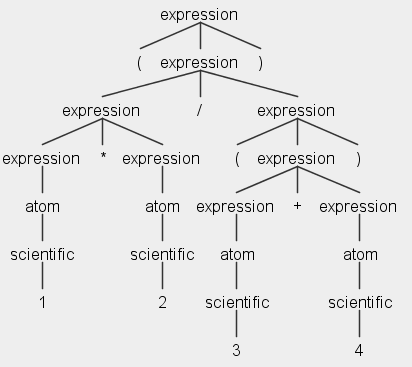
\includegraphics[scale=0.75]{images/arithmetic_syntax_tree}
	\caption{Syntax Tree of an Arithmetic Term (generated using code from \protect\cite{Everett2019})}
	\label{arithmetic_syntax_tree}
\end{figure}

\begin{figure}[p]
	\centering
	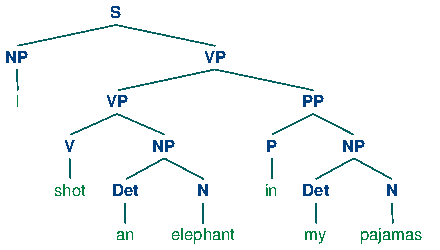
\includegraphics[scale=0.75]{images/nlp_tree}
	\caption{Syntax Tree for Natural Language Processing \protect\cite{Bird2009}}
	\label{nlp_tree}
\end{figure}

\begin{figure}[p]
	\centering
	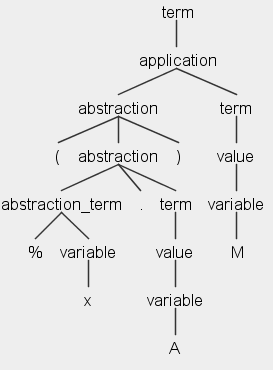
\includegraphics[scale=0.75]{images/abstract_syntax_tree}
	\caption{Lambda Calculus term $(\lambda x.A)M$ abstract syntax tree}
	\label{abstract_syntax_tree}
\end{figure}


\subsection{ANTLR}

One such tool which can help represent the structure of a term based on a particular grammar is ANTLR. ANTLR is a parsing tool which is used to build and explore syntax trees from character strings. It has a lexer to generate tokens, and has a parser to turn this stream of tokens into an abstract syntax tree which can then be evaluated using either a listener or a visitor \cite{Parr2012}. It has been used in a wide variety of contexts, including Twitter (for query parsing) and the NetBeans IDE (for parsing C++). %[is this enough of an explanation of ANTLR?]

\section{Interface}

Once a program has been created which can parse and evaluate lambda terms, an interface is needed to allow this to be used by students. The interface should be simple to understand, and as a minimum requirement should include a place for user input which will allow students to input a lambda expression alongside an output showing the resultant reduced expression. It should also include an input which will allow the user to select different types of beta-reduction, and an output which will show the typability and evaluated type of the returned expression.

\chapter{Aims and Objectives}

From the background and analysis discussed above, a set of key aims and objectives can be defined. These eight objectives have been defined below, and have been labelled with the MoSCoW system, (must-have, should-have, could-have and would-like-to-have) \cite{Agile2014}.
The program will include:

\begin{itemize}
	\item Must Have: The ability to evaluate the validity of lambda calculus terms, so students can enter terms and check whether or not they are valid. This will be done by turning the user input lambda term into an Abstract Syntax Tree using ANTLR
	\item Must have: Applied lambda calculus, to allow the input of expressions
	\item Must have: The ability to alpha convert these terms, to help students understand alpha conversion and equivalence. This will be done by navigating the abstract syntax tree generated by ANTLR
	\item Must have: Which will be contained in a web interface to allow users to use the tool easily
	\item Should have: Using beta reduction to evaluate terms to normal form to help students understand beta reduction. This will also be done by navigating the abstract syntax tree generated by ANTLR
	\item Should have: Which includes types, to help students understand types and typing rules
	\item Could have: Which offers different reduction strategies, to give students the option to understand call by value/call by need evaluation
	\item Would like to have: Which performs type inference to determine the output type of a lambda term
	\item Would like to have: And arithmetically evaluates these terms using delta reduction	
\end{itemize}

\chapter{Design and Implementation}
\section{Design}

The overall program is split into a number of distinct elements, all of which are based on the fundamental rules of Lambda Calculus as defined in previous sections.\\

Firstly, a grammar is written which defines the syntax of lambda terms and allows a term to be broken down into individual tokens. ANTLR uses this grammar to process lambda terms, creating an Abstract Syntax Tree for each incoming expression \cite{Parr2012}, a process which has been well documented and therefore will not need to be rewritten. A tree traversal mechanism is the main section of code which navigates the abstract syntax tree and performs operations to determine the resultant expression. This is the section of code which will perform the evaluation, and therefore needs to be designed accurately, with the rules of beta reduction and lambda calculus in mind. A web interface is used to house this program, giving the user a simple and convenient way to interact with the underlying system.\\

The relevant sections have been discussed below, detailing design and key decisions which needed to be made before implementation began. %WHAT TENSE IS THIS

\subsection{Grammar}

The key aim in creating this grammar was creating a syntax which sticks as closely as possible to the rules of lambda calculus. Lambda Calculus grammar is already clearly defined, with a lambda term being either a variable, an abstraction or an application \cite{Hankin2004}. Applied lambda calculus adds functions and constants to this definition \cite{Slonneger1995}, resulting in the following lambda grammar. A lambda term is one of the following:

\begin{itemize}
\item[|] An application (of form \texttt{[term] [term]})
\item[|] An abstraction (of form \texttt{[abstraction_term].[term]} where \texttt{[abstraction_term]} is defined by \texttt{$\lambda$[variable]})
\item[|] A function (of form \texttt{[term] [operation] [term]})
\item[|] A value (of form \texttt{[variable]} (the letters a-z) or \texttt{[number]} (constant))
\end{itemize}

With the addition of types, the grammar adds the option of a \texttt{:[type]} term to each variable, with each type being either a ground type (bool, int or none), or in the form \texttt{[type] $\rightarrow$ [type]}. This follows the standard syntax for typing used in the lecture material \cite{Hankin2004} \cite{Gay2019}, and consistency with this syntax allows students on the Theory of Computation course to input a lambda term directly from the lecture slides with minimal adjustment.

\subsection{Expression Evaluator}

The fundamental component of this evaluator is a tree traversal, which navigates through the token nodes and performs different operations depending on the type of node encountered. Abstractions will take an incoming value if one exists, and substitute it into the body of the abstraction. This allows an evaluated expression to be built up, and a result determined.\\

ANTLR provides two mechanisms for traversing an abstract syntax tree: listeners and visitors. A listener is a passive way of evaluating a syntax tree, used within an ANTLR Walker class which traverses the tree using a depth-first approach, triggering methods from the listener as it enters and exits each token \cite{Parr2012}. These listener methods are unable to return values, so expressions and evaluations have to be handled using separate objects within the listener class. As the walker traverses the tree, the listener builds up a running evaluation of the term, returning the result when it exits the topmost node \cite{Srivastav2017}.\\

Unlike listeners, visitors control their own traversal of the tree. By visiting the children of each node encountered explicitly, the path they take around the tree can be controlled \cite{Parr2012}. Visitors also allow custom return types, meaning nodes can return their resultant expressions directly to their parent node and do not have to rely on separate objects \cite{Srivastav2017}.\\

With beta reduction, different methods take different approaches to evaluating terms. In an application MN using a call-by-value approach, N is evaluated before M. In a call-by-need approach, N is passed into M before being evaluated. This means that depending on the type of reduction selected, the evaluator will have to traverse the tree in a different order, suggesting visitor over listener is more appropriate for this task. Furthermore, visitor methods being able to return values directly to their parents as opposed to relying on separate objects will support evaluation happening as the tree is being visited, due to the large amount of data being passed around the tree.\\

%Note to self: what tense is this section?
The visitor therefore was the main code written in this project. An ANTLR generated parser is passed to a custom visitor interface. Different visitors are defined for each of the beta-reduction strategies being implemented, since each method takes a different approach to evaluating expressions.\\

The visitor should return three separate items upon returning to the topmost node: the evaluated value of the input lambda term, whether or not the term is typable, and what type the expression will be. It will also return details of any errors where applicable, for example syntax errors which ANTLR is unable to parse, or cases where the normal form of a lambda term does not exist.

\subsection{Web Interface}

The web interface will allow the user to input a lambda term along with the type of any variable. It will also allow the user to select which reduction strategy they would like to have the term evaluated by, with call-by-need being selected as the default.\\

The code running the interface and the underlying evaluation code will be kept as separate entities, communicating through input parameters and return statements. This is to ensure the code is kept as modular as possible, allowing the evaluator code to be run using multiple different mechanisms, for example through a web interface and a command line for testing purposes. Any data the user enters will be passed to the underlying code, which will process the term and return any output via a return statement, being read and displayed to the user.

\section{Implementation}

Despite the examples in the ANTLR Reference Guide \cite{Parr2012} all being written in Java, Python was chosen as the main language for this project. ANTLR offers support for Java and Python, both of which are regularly listed in the top three programming languages being used in industry from various sources \cite{ProgLang1}\cite{ProgLang2}\cite{ProgLang3}. Since the MSc Software Development course which this dissertation is being written for teaches only Java, Python was chosen in order to expand the number of programming languages encountered throughout the course. Therefore the majority of the code for this project will be written in Python, with HTML being used for the web interface.

\subsection{Grammar}

ANTLR requires that the grammar of a language is contained in a .g4 file which defines the parser and lexer rules for lambda calculus in this case. A section of the grammar is shown in Figure \ref{parser_rules}, and indicates the parser rules for some of the token nodes, alongside the lexer rules which are shown in Figure \ref{lexer_rules}. This grammar is consistent with the syntax defined in the background section of this report, with slight modifications such as the addition of parentheses and an explicit definition for boolean and integer values.

\begin{figure}[p]
\centering
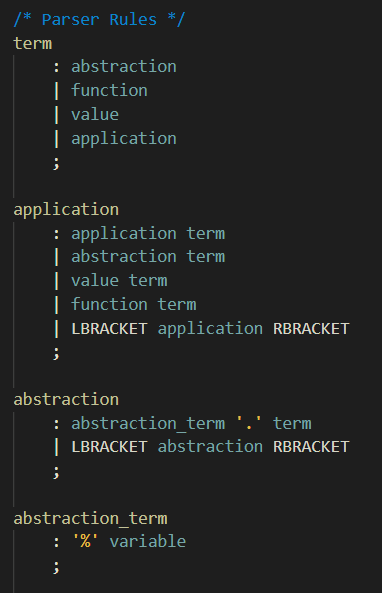
\includegraphics[scale=0.75]{images/parser_rules}
\caption{Parser Rules}
\label{parser_rules}
\end{figure}

\begin{figure}[p]
\centering
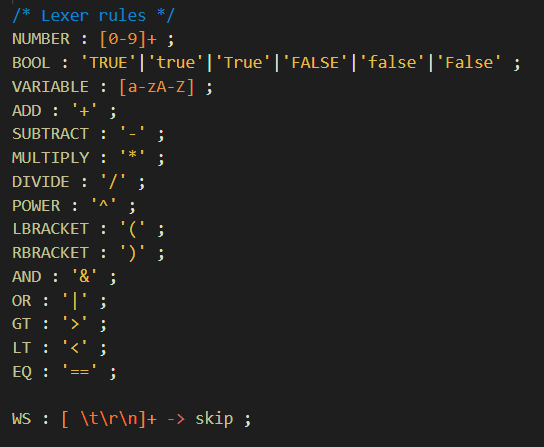
\includegraphics[scale=0.75]{images/lexer_rules}
\caption{Lexer Rules}
\label{lexer_rules}
\end{figure}

\subsection{Abstract Syntax Tree}

Having defined a grammar, ANTLR can then be used to create an abstract syntax tree, which can be seen for an example term in Figure \ref{abstract_syntax_tree_example}. This is very simple to do using ANTLR libraries, and involves passing the input term through a number of classes before passing the result through a parser which turns the tokens into an abstract syntax tree \cite{Tomassetti2007}. The lexer and parser are created by ANTLR when the grammar file is compiled, resulting in a syntax tree which processes terms based only on the syntax of the defined language.\\

The process of creating a tree from the grammar and an incoming term is well documented, and so no modifications need to be made, with the exception of attaching a custom Error Listener to both the lexer and parser, as expanded on later on in this Implementation section.

\begin{figure}[p]
	\centering
	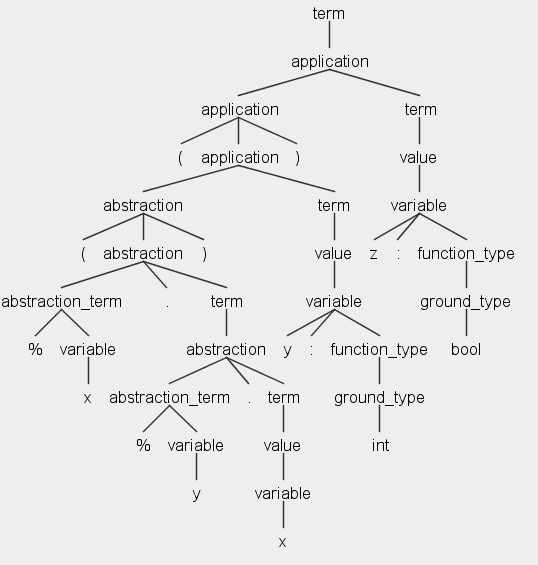
\includegraphics[scale=0.8]{images/abstract_syntax_types}
	\caption{Abstract Syntax Tree Example for (($\lambda$x.$\lambda$y.x)y:int)z:bool}
	\label{abstract_syntax_tree_example}
\end{figure}

\subsection{Expression Evaluator}
This is the largest block of code in the program, and defines how the incoming lambda term should be evaluated depending on the input given by the user. For the purposes of simplicity this code can be split into three distinct sections, alpha conversion, beta reduction and typing rules.

\subsubsection{Alpha Conversion}
The alpha conversion is based on the rules for explicit alpha conversion with substitution, as defined by \cite{Acar2008}, and as discussed in detail in a previous chapter. The final rule is the rule to be focused on and so will be repeated here for clarity:

\begin{equation*}
[t'/x](\lambda y.t)=\begin{cases}
\lambda y.t & \text{if $x=y$}\\
\lambda z.[t'/x][z/y]t & \text{if $x\ne y \land z\notin FV(t) \cup FV(t')$}
\end{cases}
\end{equation*}

This defines the process of finding a variable z that does not appear in the free variables of the incoming term or the existing term, replacing all bound variables y with this new term z, and then substituting in t’ as normal.\\

The alpha conversion code written for this project follows this process. First, the set of free variables in the term are determined, by taking the set of all alphabetic characters in the term and eliminating the bound variables. These variables are then replaced with letters that are not in the list of free variables, in situations where a clash in free variables between the two expressions are found. This produces an alpha-converted term, into which substitution can be performed using a simple \texttt{String.replace()} method in Python.

\subsubsection{Beta Reduction}

Two beta reduction strategies are taught on the Theory of Computation course, call-by-value and call-by-name. The differences between these two strategies have been discussed in detail, but the key difference is in the order in which substitution and evaluation occurs in an application MN.\\

Because of these differences in evaluation strategy, two separate visitors are used to limit the use of control coupling \cite{Lethbridge2004}. Since they share a lot of functionality, a BaseVisitor was defined which contains all common code between these two strategies. The two call-by-value and call-by-need visitors are subclassed from this base visitor, and define their unique behaviour for the application and abstraction terms.\\

The abstraction term differs between the two methods due only to typing, since determining the type of a term happens during the evaluation of that term. In call-by-value, the type of N is known before substitution, so can be carried throughout the function. In call-by-need, the whole term needs to be type checked after substitution has happened to determine the type of M with N incorporated. Two separate abstraction methods were therefore needed, with common code moved into a method defined within the base visitor.

\subsubsection{Typing Rules}

Lambda Calculus has clearly defined typing rules which are taught in the Theory of Computation course. These rules have been discussed in more detail previously. Each type can either be of ground type T, or function type T$\rightarrow$U \cite{Hankin2004}.\\

Since the visitNode methods already evaluate their children nodes, these typing rules can be integrated directly into these nodes, with each visitNode method returning a value and a type. Type checking happens throughout the code in each method where evaluation occurs, and is implemented as follows:\\

\textit{Variable}\\
Variables simply return the type given to them by the user, as defined by Rule \ref{variable_type}. Any number is given type \texttt{int}, and any boolean values TRUE or FALSE are given type \texttt{bool}.\\

\textit{Abstraction}\\
Users enter types in the form \texttt{x:type}, which can be applied to any variable included in the term. The abstraction method takes the input type T, and joins it with the output type with \texttt{->}, to become of function type \texttt{input->output}. The input and output types are either specified by the user, or determined through type inference.\\

\textit{Application}\\
For an application MN, application typing involves iteratively removing the first ground type of M and the first ground type of N until the type of N is None. For example, if M is of type \texttt{int->bool->int} and N is of type \texttt{int->bool} the typing of application MN is of type \texttt{int} through the following process:

\begin{equation*}
M:int\rightarrow bool\rightarrow int \qquad N:int\rightarrow bool
\end{equation*}
\begin{equation*}
M:bool\rightarrow int \qquad N:bool
\end{equation*}
\begin{equation*}
M:int \qquad N:None
\end{equation*}

If at any point the first ground type of N does not match the first ground type of M, the typing is invalid (for example if N was of type \texttt{bool->bool} in this case). This is implemented using string manipulation, splitting a type T into its individual ground type using the \texttt{split()} method in Python, then comparing and removing the types of M and N iteratively.\\

Type inference uses the typing rules defined above to determine the type of an output term where possible. Abstractions are initially given function type \texttt{None$\rightarrow$None}, and variables are given ground type \texttt{None}. This is inference using structural information.\\

In the visitFunction node, syntactical information can be used to determine the input and output types of terms by examining the operation term. The following is declared in code:

\begin{itemize}
	\item The operations \{\&,|\} take two boolean values and return a boolean. Therefore the type of the incoming and outgoing term can be inferred to be of type boolean
	\item The operations \{+,-,*\} take two integer values and return an integer. Similar to above, the incoming and outgoing term can be inferred to be of type integer
	\item The operations \{==,>,<\} take two integer values and return a boolean, it can therefore be inferred that the input term is of type integer, and the output is of type boolean. 
\end{itemize}

The output type of a function is used to determine the output type of its parent node. In an abstraction, this type inference can be used to determine the type of its input term, for example the lambda term $\lambda x.x+1$ can be inferred to have type \texttt{int->int} despite no input type given by the user.\\

There is a limit to this type inference, the function will infer the input type when there is only one operation term. For example, the term $\lambda x.(x==1)\&b$ contains two operations, == and \&. In this case, working out the input type is more complicated, since the typing has to be broken down in to sub-functions, which need to determine what they think the input type should be, which then needs to be examined collectively as a complete term. The type of this output is returned by the program therefore as \texttt{None->bool}. This is correct, just not as minimal as its alternative type \texttt{int->bool}.\\

While narrowing type inference to its most minimal state is definitely possible, it is not the key goal in the project, and is a small edge-case when it comes to improving student understanding. Because of this, and due to the finite nature of this project, this limitation has been deemed acceptable, with other tasks which more greatly contribute to students understanding of lambda calculus being prioritised.
%NOTE TO SELF: I need to talk abotu type inference using typing rules somewhere

\subsubsection{Error Handling}
Each visit method in the visitor returns an evaluated result and a type, which is used to build the evaluated term and determine the final result, type and type validity of the input expression.\\

However, during this process, there are a number of occurrences which could stop the program from being able to return a final result. These are broken down into two key issues: syntax errors and occurrences where a term doesn't have a normal form (and therefore cannot be evaluated to termination). These have been summarised below.\\

\textit{Syntax Errors}\\
Lambda terms often include nested parentheses. It is easy for a user to mismatch brackets, such as forgetting to close an open bracket. Because of this, before the term is passed to ANTLR, the code checks to ensure brackets are matched correctly, and if not, returns an error to the user informing them of the issue and asking them to re-enter.

Aside from this, syntax errors specific to lambda calculus are likely to occur which cannot be picked up until the term is passed through a lexer. To handle this, ANTLR's ErrorListener class is overridden, instead throwing a custom SyntaxTokenError exception which can be caught by the program and passed back to the user.\\

\textit{Recursion Errors}\\
Recursion errors are thrown in Python when a maximum stack depth is reached in order to protect Python from crashing \cite{PythonStack2019}. This is the exception which is thrown when a lambda term has no normal form, as the code keeps trying to evaluate the term before eventually throwing a RecursionError.

To handle this, the recursion limit for the code is set to 200, smaller than the python default to prevent excessive time waiting for the program to fail, but large enough to ensure that any reasonable lambda term can be processed. A recursion limit for the code equates to a lambda term with approximately 50 nested abstractions. While this is a limitation, it's is deemed to be a reasonable one, as limiting students to 50 nested abstractions as opposed to 100 is unlikely to impact student understanding. If a recursion error is thrown, it is caught by the code in a \texttt{try/except} block, and an error message informing the user that a normal form cannot be found for this term is given.

\subsubsection{Web Interface}

Flask is a web framework designed for use with Python, and allows python scripts to be controlled from a web interface \cite{FullStack2019}. The websites' front-end is written in HTML, and is connected to the python file using Flask's \texttt{render_template()} function.\\

Users enter lambda terms in the input dialogue box, entering a \% sign as a lambda symbol. Using a HTML onkeydown event, the interface automatically changes this symbol to a $\lambda$, allowing users to easily enter lambda terms. The complete web interface can be seen in Figure \ref{web_interface_no_input}, Figure \ref{web_interface_input} and Figure \ref{web_interface_error}.\\

Clicking the \textit{Check Expression} button on the web interface sends a HTTP post request to the Flask server, which takes the value held in the user input box along with the selected reduction strategy, and sends this to the main lambda program. The output is returned to the HTML code through Flask, and the webpage is re-rendered to display the results.

\begin{figure}[p]
	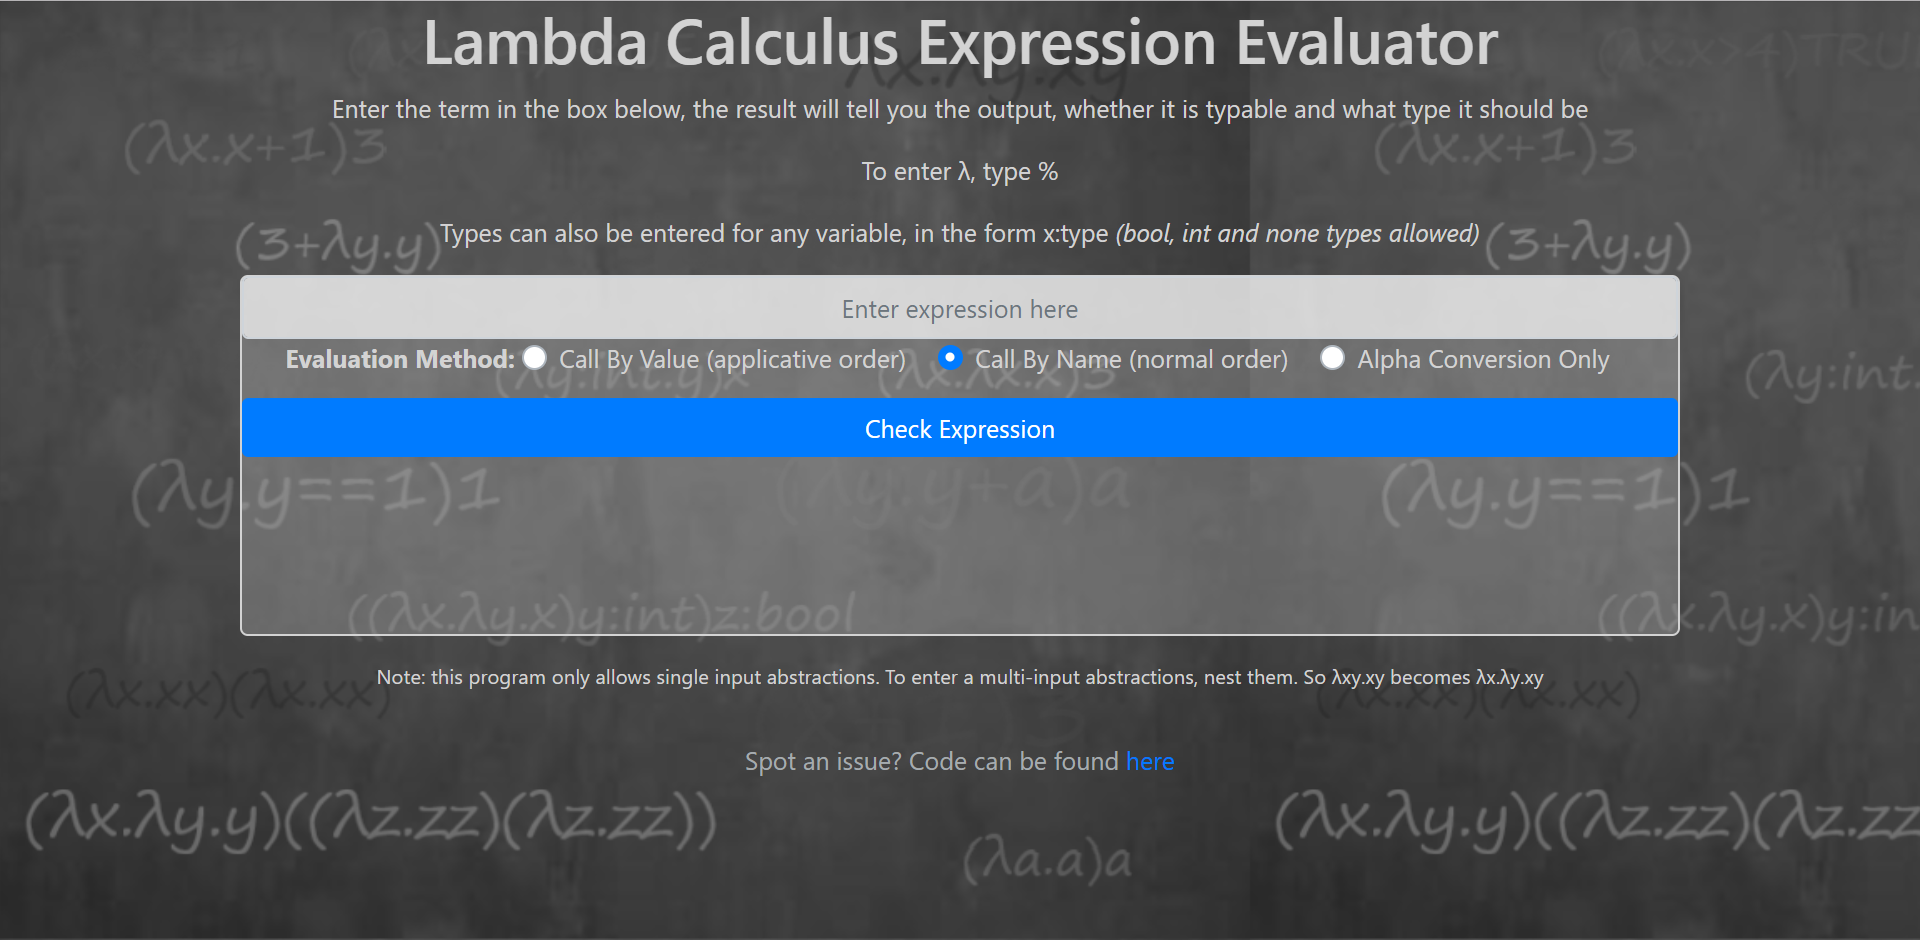
\includegraphics[scale=0.4]{images/web_interface_no_input}
	\centering
	\caption{Web Interface}
	\label{web_interface_no_input}
\end{figure}

\begin{figure}[p]
	\centering
	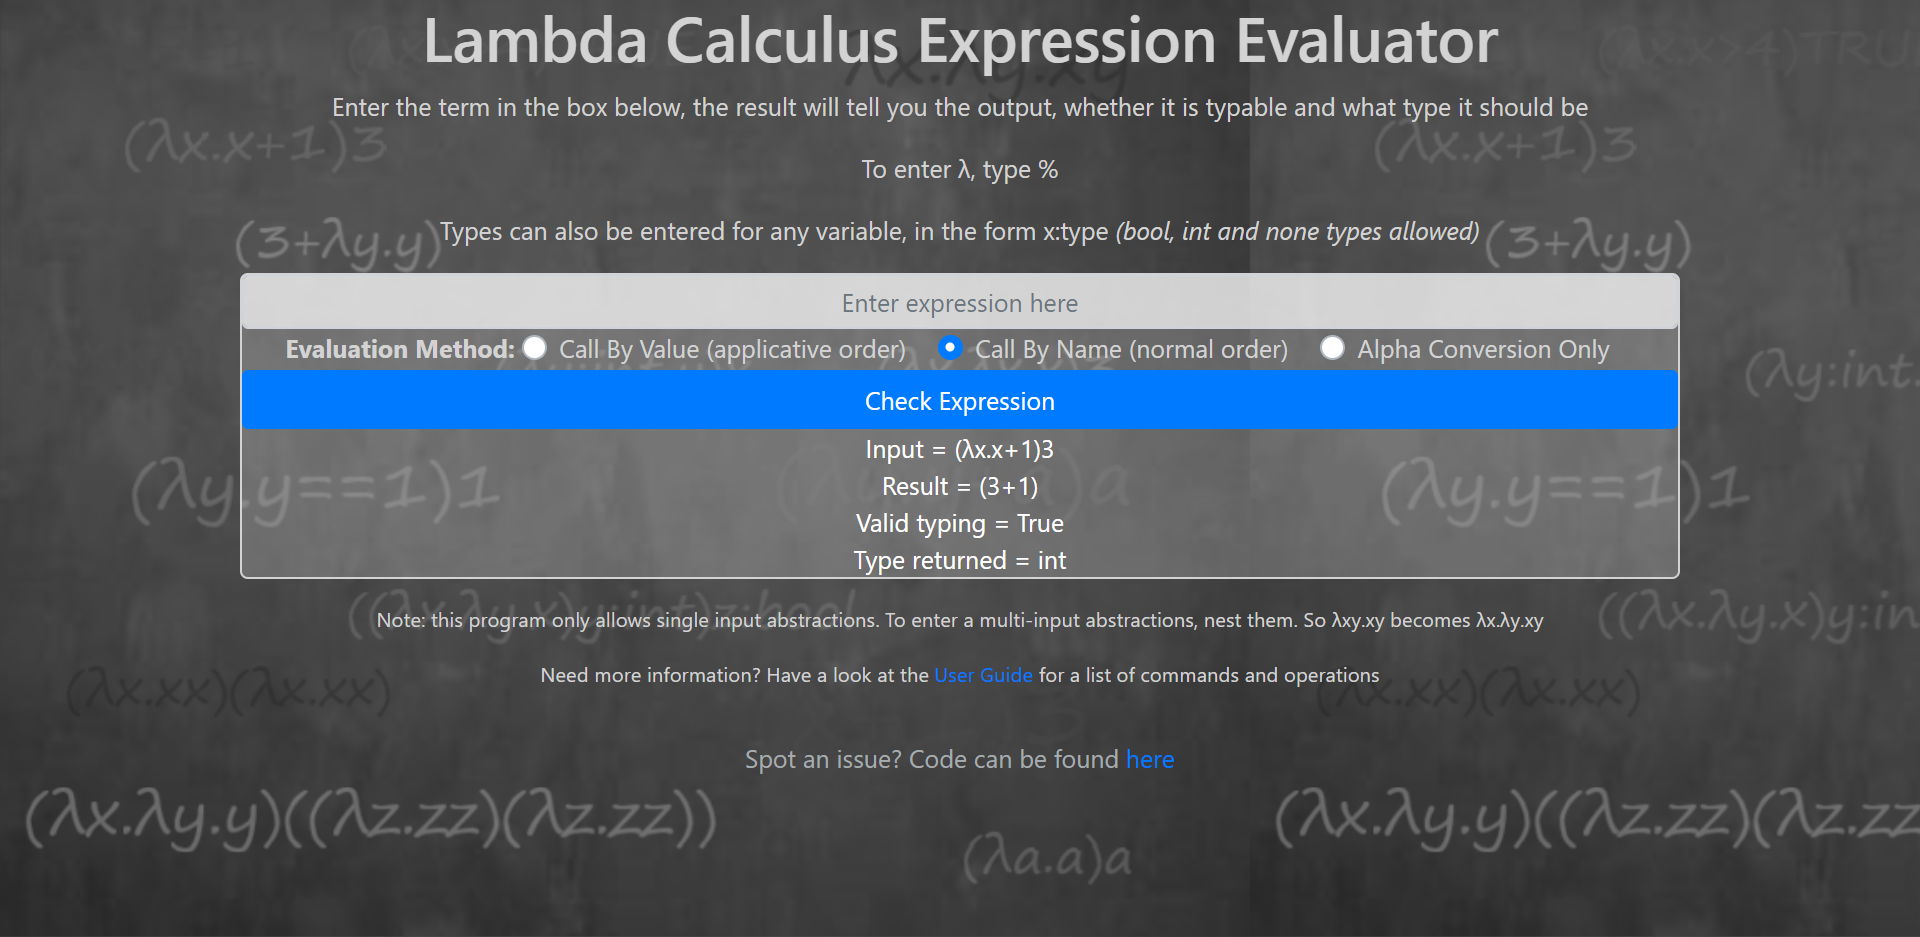
\includegraphics[scale=0.4]{images/web_interface_input}
	\caption{Web Interface With Returned Result}
	\label{web_interface_input}
\end{figure}

\begin{figure}[p]
	\centering
	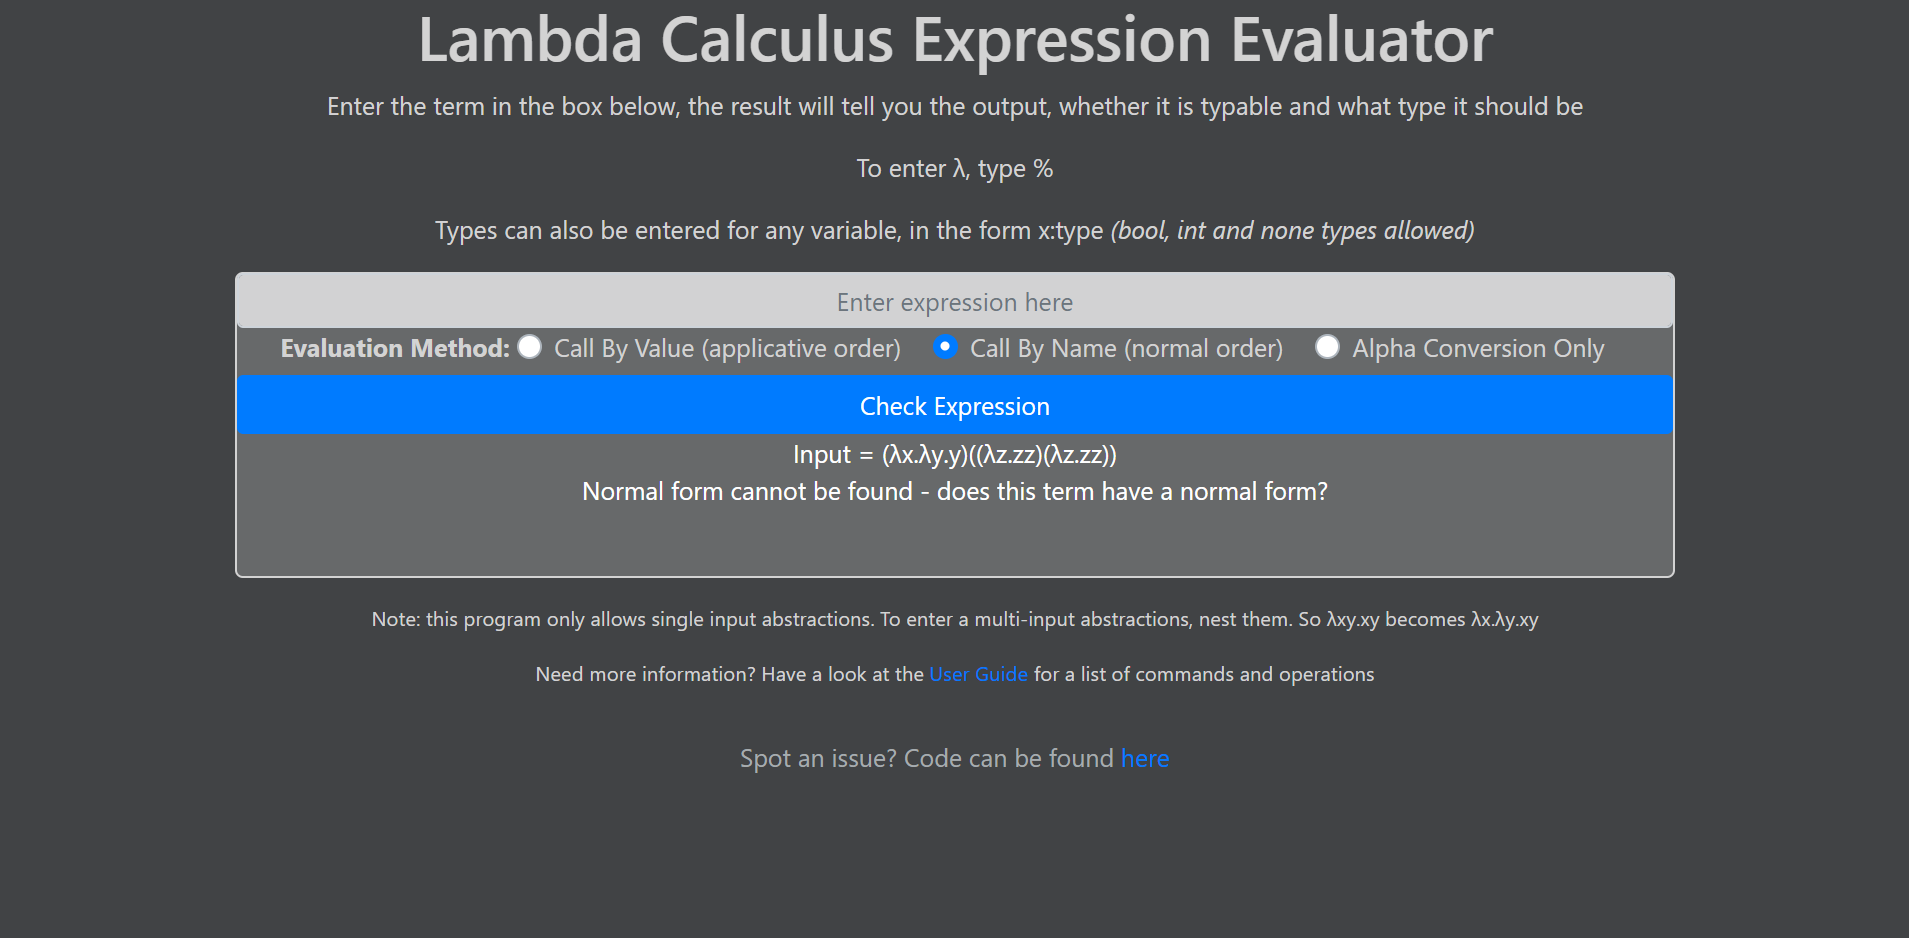
\includegraphics[scale=0.4]{images/web_interface_error}
	\caption{Web Interface With Error}
	\label{web_interface_error}
\end{figure}

\chapter{Testing}
The aim of this project is to build a web application which will verify and evaluate lambda calculus terms input by the user, with the goal of improving student understanding. This can be broken down into two key goals for the created tool, the interface should evaluate lambda terms accurately and should be useful for students learning functional programming.\\

Because of this, the testing will be broken into sections in accordance with these two goals. The first set of tests will evaluate the accuracy of the lambda term evaluation. The second set of tests will test the usability of the interface and whether or not it meets the goal of improving student understanding, by performing a user test with students who have an understanding of computer science but who have little to no knowledge of lambda calculus.

\section{Accuracy of Lambda Term Evaluation}
\label{Accuracy of Lambda Term Evaluation}
In order to test the accuracy of the evaluation, the tests were split into three categories: alpha-conversion, beta-reduction and typing rules. For each category, key points of potential failure were identified, such as multi-input lambda terms, bound variable naming clashes ($\lambda x$ being used twice in the same term testing the scope of the lambda term), order of operations issues (since applications are left-associative), and terms with no normal form.\\

All of the above were tested for, the results shown in Figure \ref{testing_log} below. The table includes the input to test, the motivation for testing that input, the expected and actual results, and an indicator showing whether or not the test was successful.\\

\begin{figure}[p]
	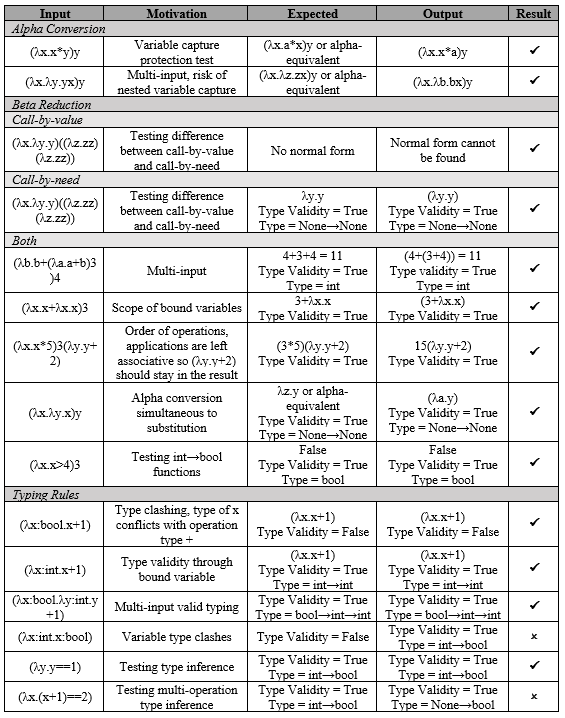
\includegraphics[scale=1.3]{images/Testing_Log}
	\centering
	\caption{Evaluating the Accuracy of Lambda Term Evaluation}
	\label{testing_log}
\end{figure}

Figure \ref{testing_log} demonstrates that in the majority of cases which have been tested, the evaluation is accurate and does yield expected results. There are a few instances where the output is not as expected, which have been discussed in greater detail in the Evaluation section of this report.

\section{Interface Usefulness and Usability}
\label{interface usefulness and usability}
\subsection{Testing}

In order to test the usability and usefulness of the interface, a user test was conducted using participants who had a computer science background but who had little to no understanding of lambda calculus. This was done in order to simulate students on the Theory of Computation course who have just been introduced to Lambda Calculus for the first time.\\

Participants were first given a Participant Information sheet and to sign a Participant Consent Form, which stated they were happy with the results of their user test to be included in this dissertation, provided their answers will be kept anonymous as will be done here. They were then asked to read a document giving them a brief introduction to lambda calculus, which was written for this test and was based on the Theory of Computation lecture slides \cite{Gay2019}. This was done to simulate students who have been introduced to lambda calculus, but are still very new to the subject.\\
%(Note to self: should I put the introduction to lambda calculus document in the appendix?)

Having read a brief summary, participants were asked to rate their understanding of lambda calculus on a scale of 1-10, before being given the interface to test. They were provided with a few sample lambda terms to test if they wanted to, but were not obligated to use them. This was to simulate students who may be using the tool to evaluate a particular lambda expression they have found in the lecture slides or online.\\

Finally, users were given a questionnaire which again asked them to rate their understanding of lambda calculus having used the interface for a short period of time, so their understanding could be compared before and after using the tool. The questionnaire also asked a number of qualitative questions, asking participants to give feedback on whether or not they would use this tool if they were studying Lambda Calculus, and what they thought of the interface.

\subsection{Results}
Although the test was not conducted with a time limit, each participant spent approximately five minutes using the interface before stating they were ready to move on. As can be seen from Figure \ref{participant_understanding}, in the five minutes participants interacted with the interface their understanding improved by 41\% on average. 100\% of participants said they would use the tool created if they were on the Theory of Computation course, and 100\% said they found it useful in improving their understanding.\\

The qualitative questions on the interface and tool revealed that participants found the system simple and easy to use, with some suggestions for improvement. Suggested interface changes included making the colour of the input box darker to differentiate between input boxes and menus, and changing the background as some participants found it distracting. Participants also suggested adding additional features such as tooltips to give the user more information on what particular lambda terms meant, and adding a workbook section which would allow users to save the results to a file in order to create a study resource they could go back to later.\\

Overall the feedback was incredibly positive, supporting the conjecture that the tool created could support student learning for those starting out with lambda calculus. Participants commented that it helped improve understanding by adding a practical element to the much more theoretical-based lecture slides.

%Note to self: should I include the results from the google survey in the appendix?

\begin{figure}[h]
	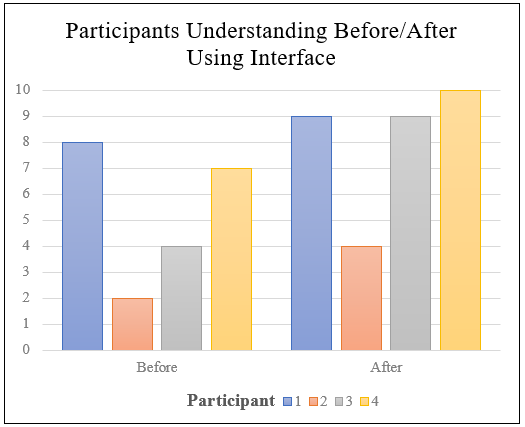
\includegraphics{images/participant_understanding}
	\centering
	\caption{Participant Understanding Results}
	\label{participant_understanding}
\end{figure}

\chapter{Evaluation}

As stated in the beginning of this report, the aim of this project is to build a web application which will verify and evaluate lambda calculus terms input by the user. This tool is created with the goal of helping future students learning functional programming to gain a better understanding of lambda calculus.

This chapter will discuss whether or not the project description has been met, and whether or not the tool created could be used as a supplementary resource for students learning lambda calculus on the Theory of Computation course taught at the University of Glasgow.

\section{Accurately Evaluating Lambda Terms}
As evidenced by section \ref{Accuracy of Lambda Term Evaluation}, the tool created does accurately evaluate lambda terms, returning the normal form, type and type validity of lambda terms for both call-by-value and call-by-need evaluation strategies. Applied lambda calculus with types is supported, as taught on the Theory of Computation Course.

\subsection{Limitations}
Figure \ref{testing_log} demonstrates some limitations with the evaluation of the final program. One such limitation is demonstrated by the $\lambda x:int.x:bool$ term with clashing types for like-terms, the results of which present this as valid typing of type \texttt{int$\rightarrow$bool}. This is because type validation within an abstraction happens at the function level when the types of variables are checked against the middle operation. The types of like-terms are not compared, an abstraction simply takes the input type (in this case \texttt{int}) and concatenates it with the output type (\texttt{bool} in this case).\\

This is a limitation, and could be fixed by giving abstractions more control over their inner terms. However, it was decided early on to keep the abstraction and the inner term as distinct as possible, a coding decision which has resulted in this fix requiring a major refactor. Because of this, the gain resulting from this edge case was not deemed high enough to warrant such a refactor in the late stage of the project, and so the limitation was left in.\\

Furthermore with typing rules, Figure \ref{testing_log} demonstrates the type inference issue when functions have multiple operations. This has been discussed in detail in the Implementation section of this report, and therefore will not be discussed here.\\

\section{Improving Student Understanding}
The user tests conducted and summarised in section \ref{interface usefulness and usability} suggest that students with a computer science background learning lambda calculus for the first time would likely find the tool useful in supporting their learning. Possible improvements such as including tooltips as suggested in user feedback are valid and would be implemented given more time.\\

The user feedback also suggested that the simplicity of the interface is a positive, and care must be taken to prevent the interface from becoming too complicated. The interface is to be used as support for the Theory of Computation lecture slides or other lambda calculus guidance as opposed to teaching those using the interface lambda calculus, and this should be maintained in any future work done.\\

With a goal of supporting learning by providing an interface which accurately evaluates lambda terms, it can be said that these goals have been met.

\section{Future Work}
Due to the time limited nature of this project, not all features or corrections have been implemented. Given more time, the following work would be done:

\begin{enumerate}
	\item Add in type-checking for like terms to prevent the same variable being given conflicting types by the user
	\item Add in multi-input abstraction terms to allow users to enter $\lambda xy.M$ as appears in the lecture slides \cite{Gay2019} as opposed to $\lambda x.\lambda y.M$
	\item Improve the type inference to allow input types of multi-operation functions to be inferred
	\item Include tooltips linked to various aspects of the web interface to give users more information
	\item Do further user testing for the web interface to get a wider understanding of any style/usability issues that exist 
	\item Allow users to enter lambda terms in the De Bruijn notation, for those unfamiliar with the Barendregt convention
\end{enumerate}

\chapter{Conclusion}
This report has documented the work done in creating a tool to evaluate lambda terms designed to support those studying the Theory of Computation at Glasgow University. The report has given an introduction to key terms, an analysis to determine specific objectives, and has detailed the design and implementation of the tool. It has also covered the testing and evaluation of the final interface to determine how well key goals have been met.\\

The outcome of the project was extremely successful, resulting in a simple and convenient tool which accurately evaluates lambda calculus terms in an easy-to-use web interface. Design decisions were made based on lecture material, but the tool was not limited so much that it could only be used by those on the Theory of Computation course. The final tool is broad enough to be accessible to those learning lambda calculus through alternate methods, but specific enough to support those on the course achieve understanding of key learning outcomes.\\

Creating this tool was very much a challenge, having no prior knowledge of lambda calculus before the project was started resulted in an extremely steep learning curve and a number of setbacks due to misunderstandings made early on in the project. As well as this ANTLR had to be learned from scratch, resulting in a portion of time being allocated to becoming familiar with the tool in order to utilise it in the best way possible.\\

Due to the finite nature of the project and the amount of learning that had to be done as implementation was underway, there are features which would benefit the tool which have not been included due to time restrictions. These include supporting multiple notations such as De Bruijn notation and multi-input terms which have been discussed previously. The tool could also be expanded in ways which would further benefit student learning, for example the option of evaluating a term step-by-step so students could see the method of evaluation explicitly, and adding tooltips to give users more guidance on the theoretical aspects of lambda calculus.\\

As well as additional features, one key goal would be to perform additional user testing across a wider demographic of participants, including those who previously have taken the Theory of Computation course, those more familiar with Lambda Calculus and those at other universities or learning lambda calculus through other means. This would help improve the tool for a wider range of potential users, and allow additional feature ideas to come from people who would actually be using it.\\

However, despite the narrow demographic of user feedback and the additional features which could potentially be implemented, the project was a huge success. From the [number of test participants] test participants, 100\% said they found the tool useful and would use it if they were on the Theory of Computation course, reporting a [statistic]\% improvement in understanding having used the tool for a short period of time. Testing has also shown that the tool does evaluate lambda terms accurately, by following the rules of lambda calculus as closely as possible and making the best use of the extremely powerful parsing tool that is ANTLR. This has resulted in a system which will accessible to students on the Theory of Computation course next year, being hosted on university servers in the near future.\\

Creating the tool was definitely a challenge, due to having no knowledge of lambda calculus or ANTLR before starting the project. But the tool created has met all the goals which were set out at the start of the project, and includes additional features going beyond the limited specification to further improve student understanding. It is hoped that future students will find this tool useful in their university studies, and that it will help to improve their understanding of lambda calculus and functional programming.

\newpage
\printbibliography

\end{document}